\section{Models}

The model architecture is adapted from the functional design of SAM,
and also informed by the development of OPUS and UrbanSim. The
functionality in SAM focuses on the allocation of land use by
sector to grid cells, from aggregate information at a mid-level
geography such as MPAs.  By reference to the UrbanSim model system,
this functionality is approximately equivalent in purpose to the
real estate development model component of UrbanSim, with some key
differences.  UrbanSim attempts to include a complete representation
of the real estate market, with occupants (consumers: households
and jobs), buildings and land (suppliers: developers and property
owners), and prices (markets: hedonic regressions representing the
interaction of suppliers and consumers).

The architecture for the model system proposed for AZ-SMART is based
on a 3-year plan, and incorporates the complete market
representation as in UrbanSim, and a multi-level geography and model
system.  We describe this in the Full Model System subsection below,
and then focus on a Phase 1 Model System in the subsequent

 section.

\subsection{Full Model System}
The full model system proposed for AZ-SMART involves some
hybridization and extension of elements of UrbanSim and SAM-IM.
Below we itemize the core elements of the full model system
architecture.  These are depicted in Figure \ref{figFlow}, which
shows the model components, their sequence of operation, and the
data objects on which the models operate.  Note that the data are
hierarchically organized in the center of the figure, with
aggregation relationships moving from bottom to top.


\begin{figure}[h]
\begin{center}
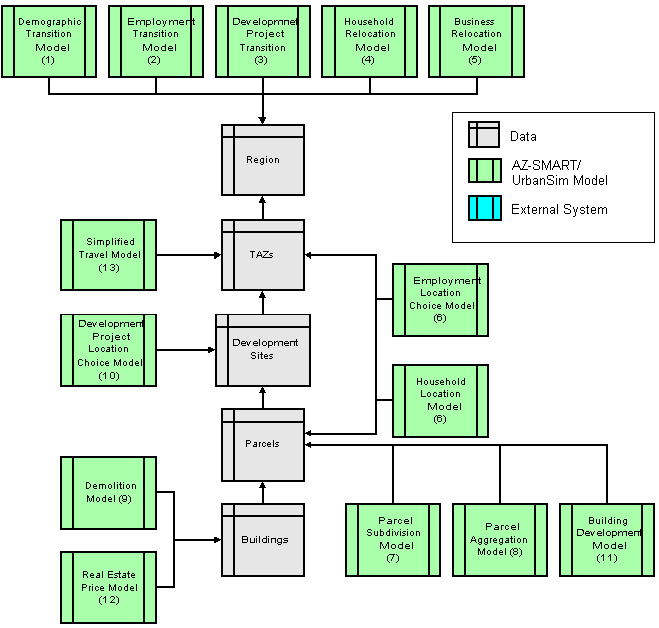
\includegraphics[scale=0.8]{figures/flow.png}
\caption{AZ-SMART Full Model Architecture} \label{figFlow}
\end{center}
\end{figure}

\begin{itemize}

\item \emph{Land-Structure-Occupant Accounting}: The full market
representation and explicit representation of and accounting of
Land-building-occupant objects and their relationship is proposed
for the full model architecture.

\item \emph{Parcels and Buildings}: Land could be represented by
parcels, land use polygons, or cells, but it is expected that
the parcel concept would be used as the principal representation
of land, and that in areas that do not have parcel data available,
land use polygons could be used in a way that treats them as
equivalent to (possibly large) parcels.  Note that there are many
to one relationships from buildings to land and from occupants to
building.  That is, a building may contain multiple occupants,
and a parcel (or land use polygon) may contain multiple buildings.
In the event that building data is not available, it could be
imputed, to preserve a consistent data model.

\item \emph{Development Projects, Sites and Templates}: Development
 Projects are proposed as a higher-level construct to represent
 one or more parcels that form a coherent single development
 project, such as single-family housing subdivision, or a shopping
 center complex.  These development projects will deal both with
 known \emph{development projects} which the user wishes to
 incorporate into the simulation, and also development projects
 predicted by the simulation and assigned to \emph{development
 sites}.  For predicted development projects, a set of pre-defined
  \emph{development templates} provide a set of configurations of
  development that include at a minimum the mix of building types
  (land uses), density, size and timetable for development.

\item \emph{Multi-level Model}: The full model system would use
a multi-level approach, incorporating parcels as the lowest level
(buildings are linked to parcels), and for the forseeable future,
one higher level geography to represent an intermediate geography
between the county and the parcel.  Traffic Analysis Zones (TAZ)
are proposed as the basis for this mid-level geography in the full
 model, simplifying the interface with the travel model system.
 There are behavioral and practical reasons for using a two-level
 geography in the model system.  Behaviorally, it is based on the
 expectation that consumers looking for a location (e.g. a household
  searching for a house) compare neighborhoods, and select properties
  to examine based on their assessment of the neighborhoods. In
  practical terms, the two-level geography provides a more convenient
  way to interface models in a modular way, for example to interface
  the travel model system, or to run the model system for corridor or
  area studies where more detail is needed in a subset of the planning
  region and less is needed outside of this focus area.

\item \emph{Microsimulation}: The proposed architecture is based on
explicit representation of the agents and objects being modeled at a
microscopic level.  Parcels, buildings, businesses (or jobs),
households, and eventually, persons (for supporting activity-based
travel models and workplace choice models and individual-level
accessibility calculations).

\item \emph{Temporal Dynamics}: The model system would be able to
use a specified time interval, such as 5-year or 1-year steps,
between which it would simulate changes to the state of each object
and agent in the system (construction of new buildings or conversion
of existing ones, movement of households and businesses from one
location to another, creation of new households or businesses).

\item \emph{Models and Interface}: A set of models will be interfaced
through a common data store, and managed by a Model Coordinator that
controls their execution and implements events (changes to the data)
proposed by models.  The individual models would be the following:

\begin{itemize}
\item Demographic Transition (Region): Reconciles the control totals
of population (by household type) with the database - adding households
to the database or removing them if a household type is declining.
\item Employment Transition (Region): Reconciles the control totals
of employment (by sector) with the database - adding businesses (jobs)
to the database or removing them if a sector is declining.
\item Development Project Transition (Region): Reconciles the total
demand for real estate by type, including the results of the Demographic
and Employment Transition models, with the existing stock of real estate,
by generating proposed Development Projects until vacancy rates reach
long-term structural levels.
\item Household Relocation (Region): Predicts whether a household will
move from their existing residence during the next time step.
\item Business Relocation (Region): Predicts whether a business  (job)
will move from their existing location during the next time step.
\item Household Location (TAZ and Parcel): Predicts the building that
a new or moving household will choose from among the set of buildings
with a vacanct unit.
\item Business Location (TAZ and Parcel): Predicts the building that a
new or moving business (job) will choose from among the set of buildings
with sufficient vacanct space.
\item Parcel Subdivision (Parcel): Predicts the number and size of
parcels to create from a large parcel that is to be subdivided to create
a development project. Depending on whether the project is known or
predicted this will use information provided in the development project
description or drawn from a development template.
\item Parcel Aggregation (Parcel): Combines adjacent parcels to create
a \emph{development site} suitable to place a development project.
\item Demolition (Building): Removes existing buildings based on age
and other characteristics that would indicate a high probability to
convert to another use or be abandoned.
\item Development Project Location (Development Site): Predicts the
development site chosen to locate a development project.
\item Building Development Model (Parcel): This would be based on the
Development Velocity Model, and predicts the construction of individual
buildings on parcels within a development project.
\item Real Estate Price Model (Building): This will predict the price
per unit (or sqft) for each type of real estate at each location (parcel).
\item Simplified Travel Model (TAZ): An abbreviated travel model with
just a.m. peak, and other simplifications to provide a relatively
high-speed regional travel model to use in intermediate years preceding
the target year for the regional transportation plan.
\end{itemize}
\end{itemize}

The models proposed for implementation in Phase 1 of this project are
described in greater detail in the following section.

\subsection{Phase 1 Model System}
Phase 1 of the AZ-SMART project focuses on the allocation of land use
sectors, essentially the real estate development process.  The plan
for Phase 1 is to focus on the real estate development components of
the full model system described in the preceding section, and to
suppress or use only simple 'stub' models for the remaining models
in the full system.  The objective is to provide the functionality
that is provided now by SAM, but in an implementation that is a
very big step towards a fully integrated market simulation model
system such as UrbanSim, and incorporating valuable innovations
such as the management of known development projects, and the use
of an intermediate level geography such as RAZ as the basis for
control totals for allocation to parcels (or land use polygons).

The following models would be the focus of model development in Phase 1:

\begin{itemize}
\item Parcel Subdivision (Parcel)
\item Parcel Aggregation (Parcel)
\item Development Project Location (Development Site)
\item Building Development Model (Parcel)
\item Real Estate Price Model (Building)
\item Travel Model Interface (current emme/2 or new TransCad model)
\end{itemize}

The following models would be implemented for completeness, but would
use only the simplest specification, to allow completeness.  For example,
the household location choice model could use an empty specification,
which would randomly allocate the household control total for a RAZ to
the housing units that have been developed on parcels in the RAZ.

\begin{itemize}
\item Demographic Transition (RAZ)
\item Employment Transition (RAZ)
\item Development Project Transition (RAZ)
\item Household Location (Parcel)
\item Business Location (Parcel)
\end{itemize}

The components of the full model system would be deferred until after Phase 1:

\begin{itemize}
\item Demolition (Building)
\item Simplified Travel Model (TAZ)
\end{itemize}


\subsection{Anatomy of the Development Project Location Model}
As the core model of the phase 1 model effort, the Development Project Location Model warrants
further detailing here.  The proposed model architecture has the following steps, using a 5-year time interval \footnote{Note: this is a modification of the approach proposed in the first meeting,
incorporating feedback from the first meeting}.

\subsubsection{Determine Quantity of Development Needed}

The first task is to translate mid-level model predictions of population and employment by RAZ (or
other mid-level geography) into predicted demands for housing units and land area of non-residential
uses by type. This would be done using average density and occupancy assumptions.

\subsubsection{Determine Development from Active Projects}

Compute the quantity of development expected in a RAZ (or other mid-level geography) for each land use
sector based on the velocity within Active Development projects. Assign the development generated
by Active Development Projects to the parcels (or polygons) within those developments.

\subsubsection{Determine Eligible Development Sites}

Evaluate parcels (polygons) with vacant land to determine what kinds of development would be
permitted on them
according to the development constraints represented by Planned Land Use and other constraints
(slopes, etc).  This applies development constraints in order to produce Eligible Vacant Lands for
development. Evaluate potential availability of Redevelopment Districts for new development.

Generate \emph{development sites} from 'patches' of available land suitable for development.
These are
areas formed by contiguous parcels or polygons eligible for development for a particular land use
sector, and would serve as a counterpart to the polygons digitized by users for planned and active
development projects.  They would allow the comparable representation of Development Sites from all
sources.

\subsubsection{Generate Development Templates}
Here we propose to generate a set of somewhat standardized templates to apply to new development
projects simulated by the model (not the known development projects), which specify the land area,
land use, number of residential units, number of building square feet, development velocity function,
and development cost.  Other characteristics could be added to templates, but these would be enough
to begin.  The number of templates could be extended over time.  Values of the template could also
be given as a range, or with some degree of flexibility, to allow their adaptation to existing parcels
or land use polygons that do not conform to the shape of existing available polygons.

\subsubsection{Generate Development Projects}

Next, we would evaluate for each development site the applicable development constraints, and
generate a set of proposed \emph{development projects}, from the set of \emph{development templates}
that could be developed on each \emph{development site} according to the current \emph{development
constraints}.  Note that there may be more than one project that would be allowed on a site, and
there may be sites that would not allow any projects to be developed.  The result of this step
would be a list of potential development projects, from which the most likely projects should be
selected, while imposing the constraint that once a project is selected for a site, the site is
excluded from further consideration for other projects, and that once the project committments
reach a stage that at completion they would cause the vacancy rate in a given property type (land
use) to exceed a long-term stable rate (a break-even rate for developers), a project will not be
accepted for development.  This is equivalent to the role of the financial sector providing
capital to developers for financing construction projects. When vacancy rates exceed a long-term
level that is seen as a high-risk threshold, the likelihood of being able to secure financing for
a development project should fall quickly.

\subsubsection{Estimate Profit}
The evaluation of which projects will be successful in securing financing is likely to be proportional
to their expected profit.  Simply put, the expected profit is a reasonable measure of the relative
probability of one project being developed as compared to other potential projects.  Note that this
approach combines and reconciles the two contrasting approaches used in real estate economics and
finance: the site looking for a use (the landowner perspective) and the use looking for a site (the developer perspective).  If we generate possibly multiple project proposals on each development site,
and then compare their expected profit not only across proposals for the same site, but also across
sites, then we have an approach that accounts for the competition among developers for sites, and
among land owners for development.  Note that this is a significant advance over the current
specification of both UrbanSim and SAM-IM.

We can estimate the expected profit by a fairly straightforward method: hedonic regression.  This
approach is already well supported in OPUS and UrbanSim, and allows the specification and estimation
of models with price as the dependent variable (or log price), and a set of structural and locational
attributes on the right hand side of the model.  It essentially 'decomposes' the sales transaction
price (or assessed value if sales data are not readily available) into component marginal prices for
each attribute, such as bedrooms, square footage, age, accessibility and other locational
and structural characteristics.

Using hedonic price models for each property type, we can estimate the resulting final value of any
development project by predicting the valuation of the component parts of a project and summing them
over the components.  If we subtract the value of the site prior to development, and subtract the
cost of the construction (and possibly the cost of demolishing existing buildings on the site), then
we have a working estimate of the expected profit from the development.

\subsubsection{Predict Development Project Proposal Probabilities}
Once the development project proposals have been evaluated and the expected profit from each has been
estimated, we can use a simple multinomial logit model to generate the probabilities of each being
developed.  The only term in the utility function is the expected profit, and the probability of
development will be proportional to the relative profit of the proposed project.

\subsubsection{Sample Development Projects Until Demand Met}
Once we have generated the probability distribution across projects, we may use that to sample from.
We draw samples from the probability distribution and add them to the list of committed projects,
at each step updating the amount of committed space by type, and evaluating whether we have reached
a cutoff threshold for any property types.  Once the committed projects reach a point that the next
project adds enought space to exceed the structural vacancy rate, then the algorithm will reject any
additional proposals that would further increase the vacancy rate in that property type.  The drawing
process proceeds until the threshold vacancy rate has beeen exceeded in all property types or a
predefined number of iterations has been reached.

\subsubsection{Iterate over RAZs (or other geography) and Allocate Unplaced Development Projects}

Once allocation of all development in a RAZ or other mid-level geography is completed, process the
next RAZ. If not all development could be allocated in a RAZ, accumulate unmet demand within a higher
level geography to be processed in a final iteration. If needed, allocate unmet demand from higher
level (MPA for example), to Development Sites as above.
